\documentclass[12pt]{article}

\usepackage[utf8]{inputenc}
\usepackage[T1]{fontenc}
\usepackage[spanish]{babel}
\usepackage{lmodern}
\usepackage{graphicx}
\usepackage{eso-pic}
\usepackage{xcolor}
\usepackage{booktabs}
\usepackage{caption}
\usepackage[
  paperwidth=84.1cm,
  paperheight=118.9cm,
  left=3cm,
  right=3cm,
  top=21cm,
  bottom=12cm
]{geometry}

\definecolor{navy}{HTML}{123D5B}
\definecolor{gold}{HTML}{C38B2D}

\AddToShipoutPictureBG*{%
  \AtPageLowerLeft{%
    
\includegraphics[width=\paperwidth,height=\paperheight]{fondo.pdf}%
  }%
}

\pagestyle{empty}
\setlength{\parindent}{0pt}
\setlength{\parskip}{0.7em}
\renewcommand{\familydefault}{\sfdefault}
\DeclareCaptionFont{posterlarge}{\fontsize{22}{27}\selectfont}
\captionsetup{font=posterlarge,labelfont=bf}

\newcommand{\postersection}[1]{%
  \vspace{0.6cm}%
  {\color{navy}\fontsize{38}{45}\selectfont\bfseries #1\par}%
  \vspace{0.2cm}%
  {\color{gold}\rule{\linewidth}{2pt}}%
  \vspace{0.35cm}%
}

\newcommand{\postercolumnsection}[1]{%
  \vspace{0.6cm plus 1fill}%
  {\color{navy}\fontsize{38}{45}\selectfont\bfseries #1\par}%
  \vspace{0.2cm}%
  {\color{gold}\rule{\linewidth}{2pt}}%
  \vspace{0.35cm}%
}

\begin{document}
\color{black}
\fontsize{30}{39}\selectfont

\begin{center}
  {\color{navy}\fontsize{68}{78}\selectfont\bfseries Título del trabajo\par}
  \vspace{0.4cm}
  {\fontsize{32}{38}\selectfont Nombre Apellido\textsuperscript{1}, Nombre Apellido\textsuperscript{2}\par}
  {\fontsize{24}{30}\selectfont
    \textsuperscript{1}Institución o departamento \quad
    \textsuperscript{2}Institución o departamento\par}
\end{center}

\vspace{0.8cm}
\postersection{Resumen}
Este póster presenta un ejemplo de evaluación del semirango de steering
BF-suitable en función de la frecuencia. La curva de la Figura~\ref{fig:steering}
se compara con un requisito de referencia de 45\textdegree{} para identificar
intervalos de operación potencialmente adecuados. En el punto señalado de
4.375\,GHz, la gráfica muestra un semirango aproximado de 48\textdegree{}; la
lectura es visual y debe confirmarse con los datos originales del análisis.

\vspace{0.5cm}
\begin{minipage}[t][62cm][s]{0.48\textwidth}
  \postercolumnsection{Introducción}
  En un arreglo de antenas, el patrón de radiación del elemento y su variación
  con la frecuencia influyen en la dirección y cobertura del haz. El análisis y
  modelado de patrones de elementos Vivaldi es un antecedente útil para evaluar
  arreglos lineales\cite{Nurhayati2019}. Aquí se ilustra una métrica
  complementaria: el máximo semirango angular que satisface la condición
  BF-suitable.

  El objetivo del ejemplo es contrastar esa métrica con un umbral de
  45\textdegree{} y destacar una frecuencia de interés, sin inferir resultados
  fuera de los que aparecen en la gráfica.

  \postercolumnsection{Metodología}
  Se representa el semirango BF-suitable (eje vertical) frente a la frecuencia
  (eje horizontal). La línea discontinua indica el requisito de
  45\textdegree{}; los tramos de la curva que alcanzan o superan esa línea
  cumplen visualmente el criterio. La estrella marca 4.375\,GHz. Para un estudio
  reproducible, sustituye esta descripción por el método de cálculo, la
  configuración del arreglo, las condiciones de simulación o medición y la
  incertidumbre correspondiente.

  \postercolumnsection{Figura de ejemplo}
  La Figura~\ref{fig:steering} se carga desde el archivo local
  \texttt{Fig01.png}. Para añadir otra imagen, copia el archivo a esta carpeta y
  cambia el nombre dentro de \texttt{\string\includegraphics}; ajusta el ancho
  con \texttt{width=\string\linewidth} o con una fracción como
  \texttt{width=0.8\string\linewidth}.

  \begin{center}
    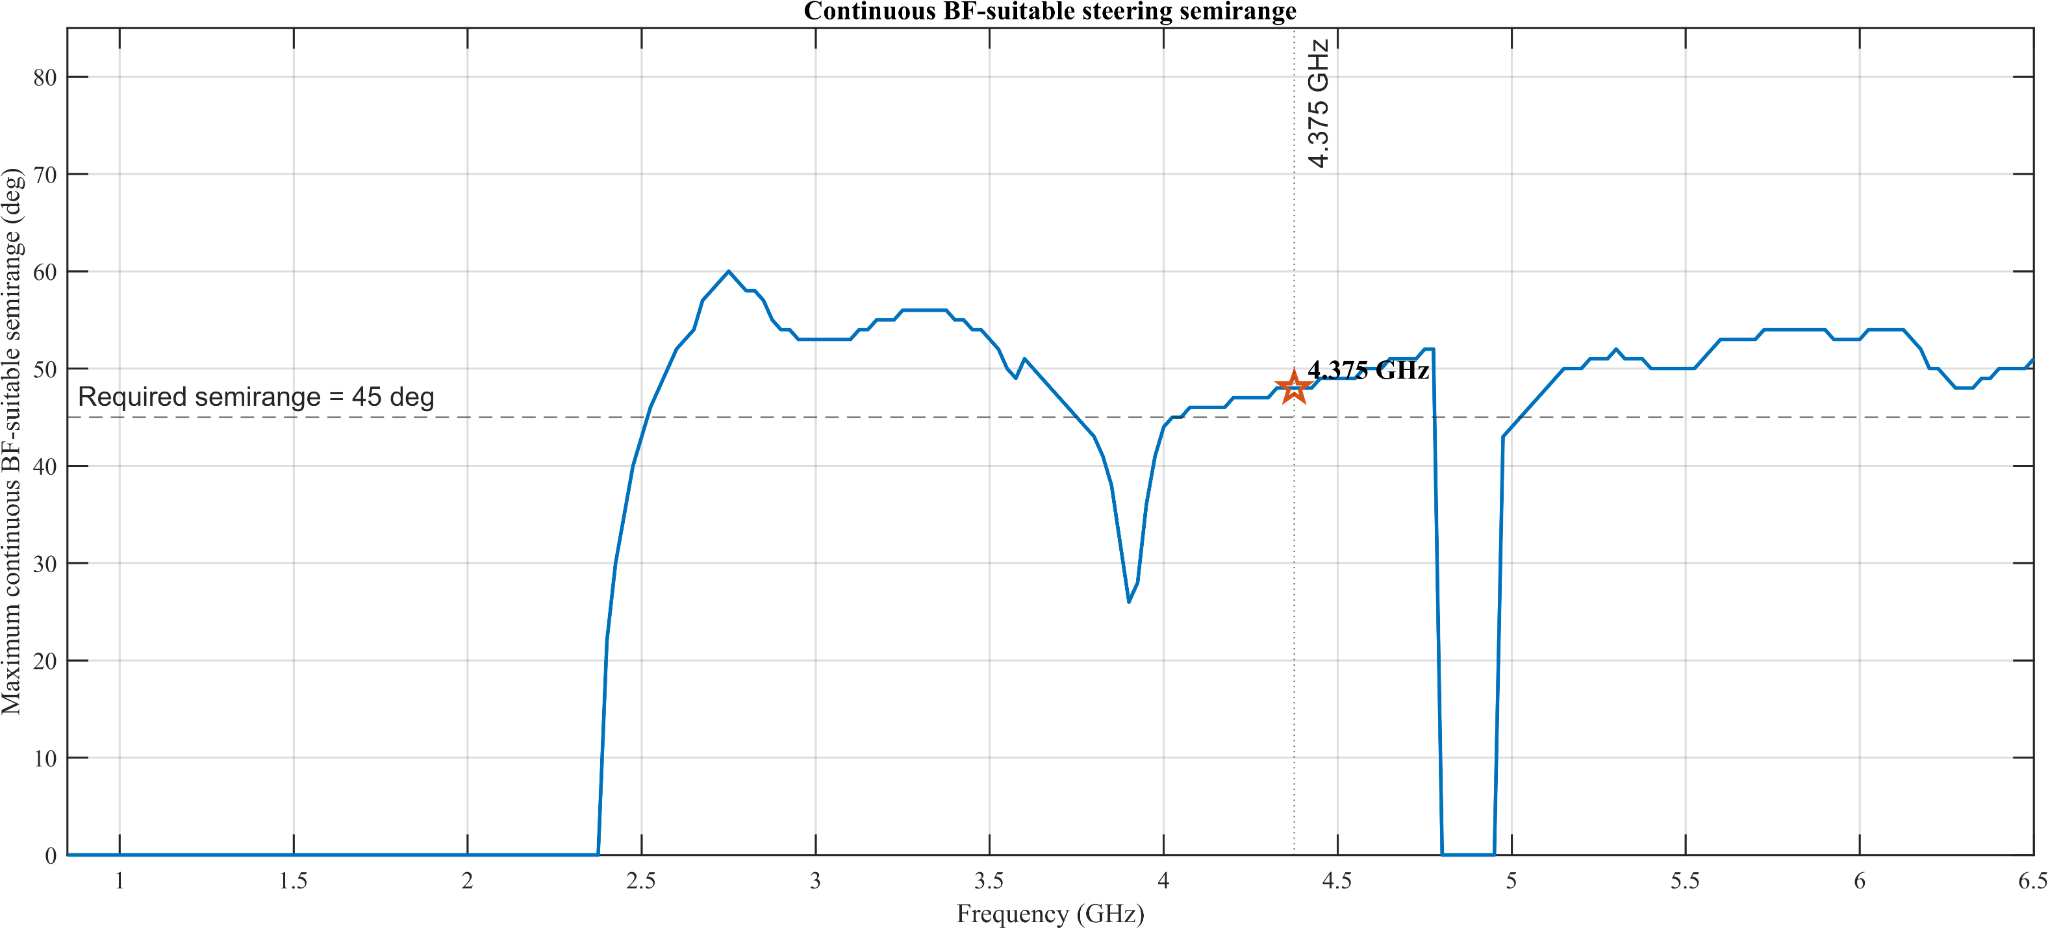
\includegraphics[width=\linewidth]{Fig01.png}
    \captionof{figure}{Semirango BF-suitable continuo en función de la frecuencia.
      La línea discontinua representa el requisito de 45\textdegree{} y la estrella
      señala 4.375\,GHz.}
    \label{fig:steering}
  \end{center}
\end{minipage}\hfill
\begin{minipage}[t][62cm][s]{0.48\textwidth}
  \postercolumnsection{Resultados}
  En la frecuencia marcada, la curva se sitúa aproximadamente en
  48\textdegree{}, unos 3\textdegree{} por encima del umbral de
  45\textdegree{}. La gráfica también contiene regiones con valores inferiores
  al requisito, por lo que la frecuencia por sí sola no describe todo el
  comportamiento de banda; conviene examinar los intervalos completos y sus
  discontinuidades.

  \begin{center}
    \captionof{table}{Lectura aproximada del punto destacado en la Figura~\ref{fig:steering}.}
    \label{tab:ejemplo}
    {\fontsize{20}{25}\selectfont
    \begin{tabular}{p{0.43\linewidth}p{0.22\linewidth}p{0.25\linewidth}}
      \toprule
      Indicador & Requisito & Lectura gráfica \\
      \midrule
      Frecuencia destacada & -- & 4.375\,GHz \\
      Semirango BF-suitable & $\geq 45^\circ$ & $\approx 48^\circ$ \\
      Margen respecto al requisito & $\geq 0^\circ$ & $\approx 3^\circ$ \\
      \bottomrule
    \end{tabular}}
  \end{center}

  \postercolumnsection{Discusión}
  El punto señalado supera visualmente el umbral, pero esta observación aislada
  no demuestra que toda la banda sea adecuada. La tabla resume únicamente una
  lectura aproximada de la figura; para reportar resultados definitivos, usa
  valores exportados de los datos y especifica el criterio BF-suitable aplicado.

  \postercolumnsection{Conclusiones}
  El ejemplo muestra cómo comparar una métrica angular con un requisito y
  comunicar un punto de operación mediante una figura y una tabla. La
  verificación final debe basarse en los datos del análisis y en las
  especificaciones del sistema.

  {\fontsize{20}{26}\selectfont
  \renewcommand{\refname}{\color{navy}\fontsize{38}{45}\selectfont\bfseries Referencias}
  \begin{thebibliography}{1}
    \bibitem{Nurhayati2019} Nurhayati, E. Setijadi, and G. Hendrantoro,
    ``Radiation pattern analysis and modelling of coplanar Vivaldi antenna
    element for linear array pattern evaluation,'' \emph{Prog. Electromagn.
    Res. B}, vol. 84, pp. 79--96, 2019, doi: 10.2528/PIERB19040502.
  \end{thebibliography}}
\end{minipage}

\end{document}